\section{Database Design}

\subsection{Database design goals}

The PizzaHUST database is designed to support the complete business lifecycle of the system: user identity, catalog management, customization options, combo promotions, cart persistence, order creation, order tracking, kitchen prioritization, reporting support, and external-delivery synchronization. In practical terms, the schema must support both the \emph{designed full scope} of the project and the \emph{current implementation reality} captured in the repository.

Two database design requirements are especially important:

\begin{itemize}
    \item the schema must represent both guest orders and registered-customer orders;
    \item the schema must preserve historical order meaning even when live catalog data changes later.
\end{itemize}

These requirements explain several later design decisions, especially nullable user ownership on orders and snapshot storage for selected options.

\subsection{Conceptual ERD and evolved implementation schema}

The project includes an early DBML design derived from the Week 1 ERD and data-dictionary work. That early model captures the main business entities, but the implemented schema has evolved through migrations as the project moved from initial analysis to runnable application behavior.

This distinction matters for the report:

\begin{itemize}
    \item the DBML and early ERD describe the \emph{initial conceptual structure};
    \item the SQLAlchemy models and Alembic migrations describe the \emph{current evolved schema};
    \item the final report should acknowledge that the schema evolved, then present ERD figures regenerated from the current logical design rather than from the outdated draft alone.
\end{itemize}

For example, the current codebase includes category-owned option groups, combo choice slots, cart persistence, webhook idempotency, image galleries, loyalty accrual fields, tracking-note sources, and operational settings tables that do not all appear in the initial DBML snapshot.

\subsection{Entity groups and relationships}

Table~\ref{tab:database-entities} summarizes the main entity groups in the current design.

\begingroup
\small
\setlength{\LTpre}{0.4em}
\setlength{\LTpost}{0.8em}
\captionof{table}{Database entity groups and design purpose}\label{tab:database-entities}
\begin{tabular}{L{0.19\linewidth} L{0.35\linewidth} L{0.38\linewidth}}
\toprule
\textbf{Entity group} & \textbf{Main tables} & \textbf{Purpose} \\
\midrule
Identity and roles & \texttt{users} & Stores customer, admin, and kitchen identities, phone-based login data, profile data, roles, and loyalty totals. \\
Catalog structure & \texttt{categories}, \texttt{products}, \texttt{product\_images} & Organizes products, pricing baselines, activation state, and gallery images. \\
Customization model & \texttt{option\_groups}, \texttt{options}, \texttt{product\_options} & Defines reusable option groups and per-product option enablement. \\
Combo model & \texttt{combos}, \texttt{combo\_items}, \texttt{combo\_images} & Represents promotional bundles, timing windows, choice slots, and combo imagery. \\
Cart model & \texttt{carts}, \texttt{cart\_lines} & Stores server-side cart state for guest or authenticated users. \\
Order model & \texttt{orders}, \texttt{order\_items}, \texttt{order\_item\_options} & Stores placed orders, line items, combo decomposition, and historical selection snapshots. \\
Tracking and workflow audit & \texttt{order\_tracking}, \texttt{webhook\_events} & Records order-state history and protects delivery callbacks against duplicate processing. \\
Operational read/support data & \texttt{kitchen\_queue\_view}, \texttt{business\_settings}, \texttt{delivery\_ward\_fees} & Supports kitchen prioritization and configurable runtime business values. \\
\bottomrule
\end{tabular}
\endgroup

\subsection{Relationship overview}

To keep the schema readable in the report, the current database design is shown through one complete logical ERD and several smaller focused ERD views. The first figure gives full-schema coverage, while the later figures isolate the catalog/option model, the combo model, and the order/workflow model.

\begin{figure}[htbp]
    \centering
    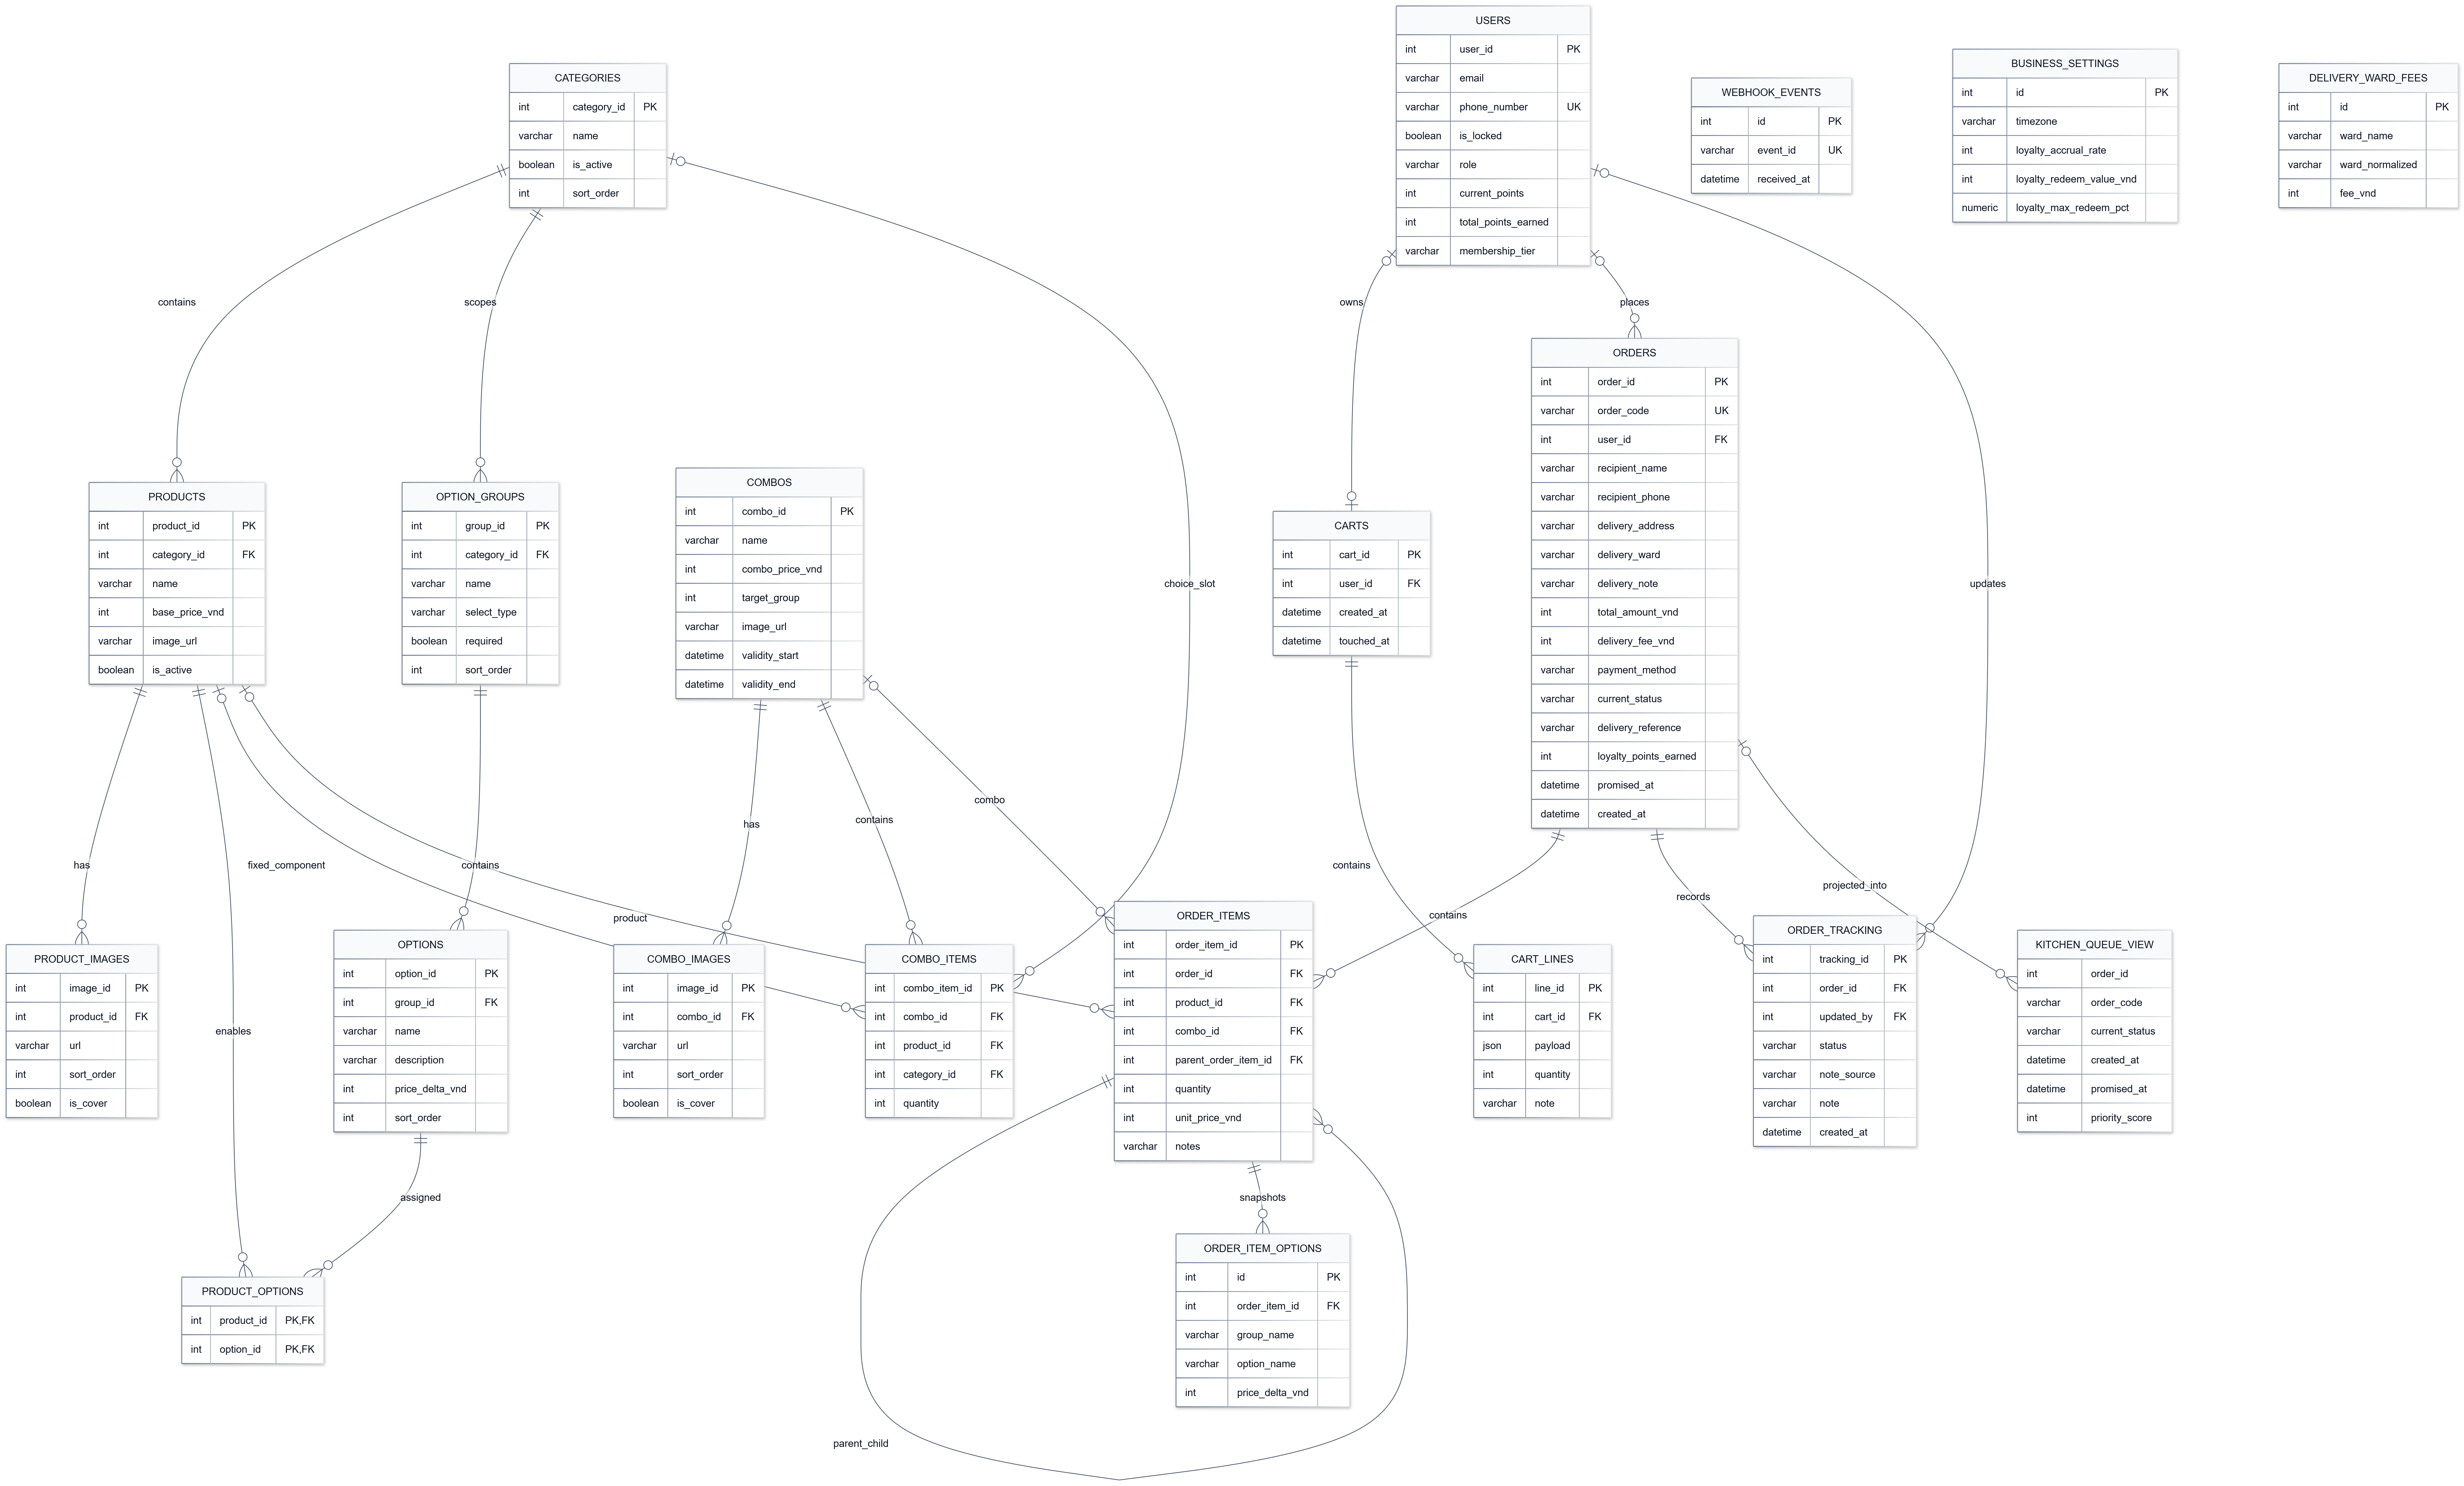
\includegraphics[width=\textwidth,height=0.84\textheight,keepaspectratio]{latex_report/figures/database_overview_full.png}
    \caption{Complete current logical ERD of PizzaHUST}
    \label{fig:database-overview-full}
\end{figure}

\begin{figure}[htbp]
    \centering
    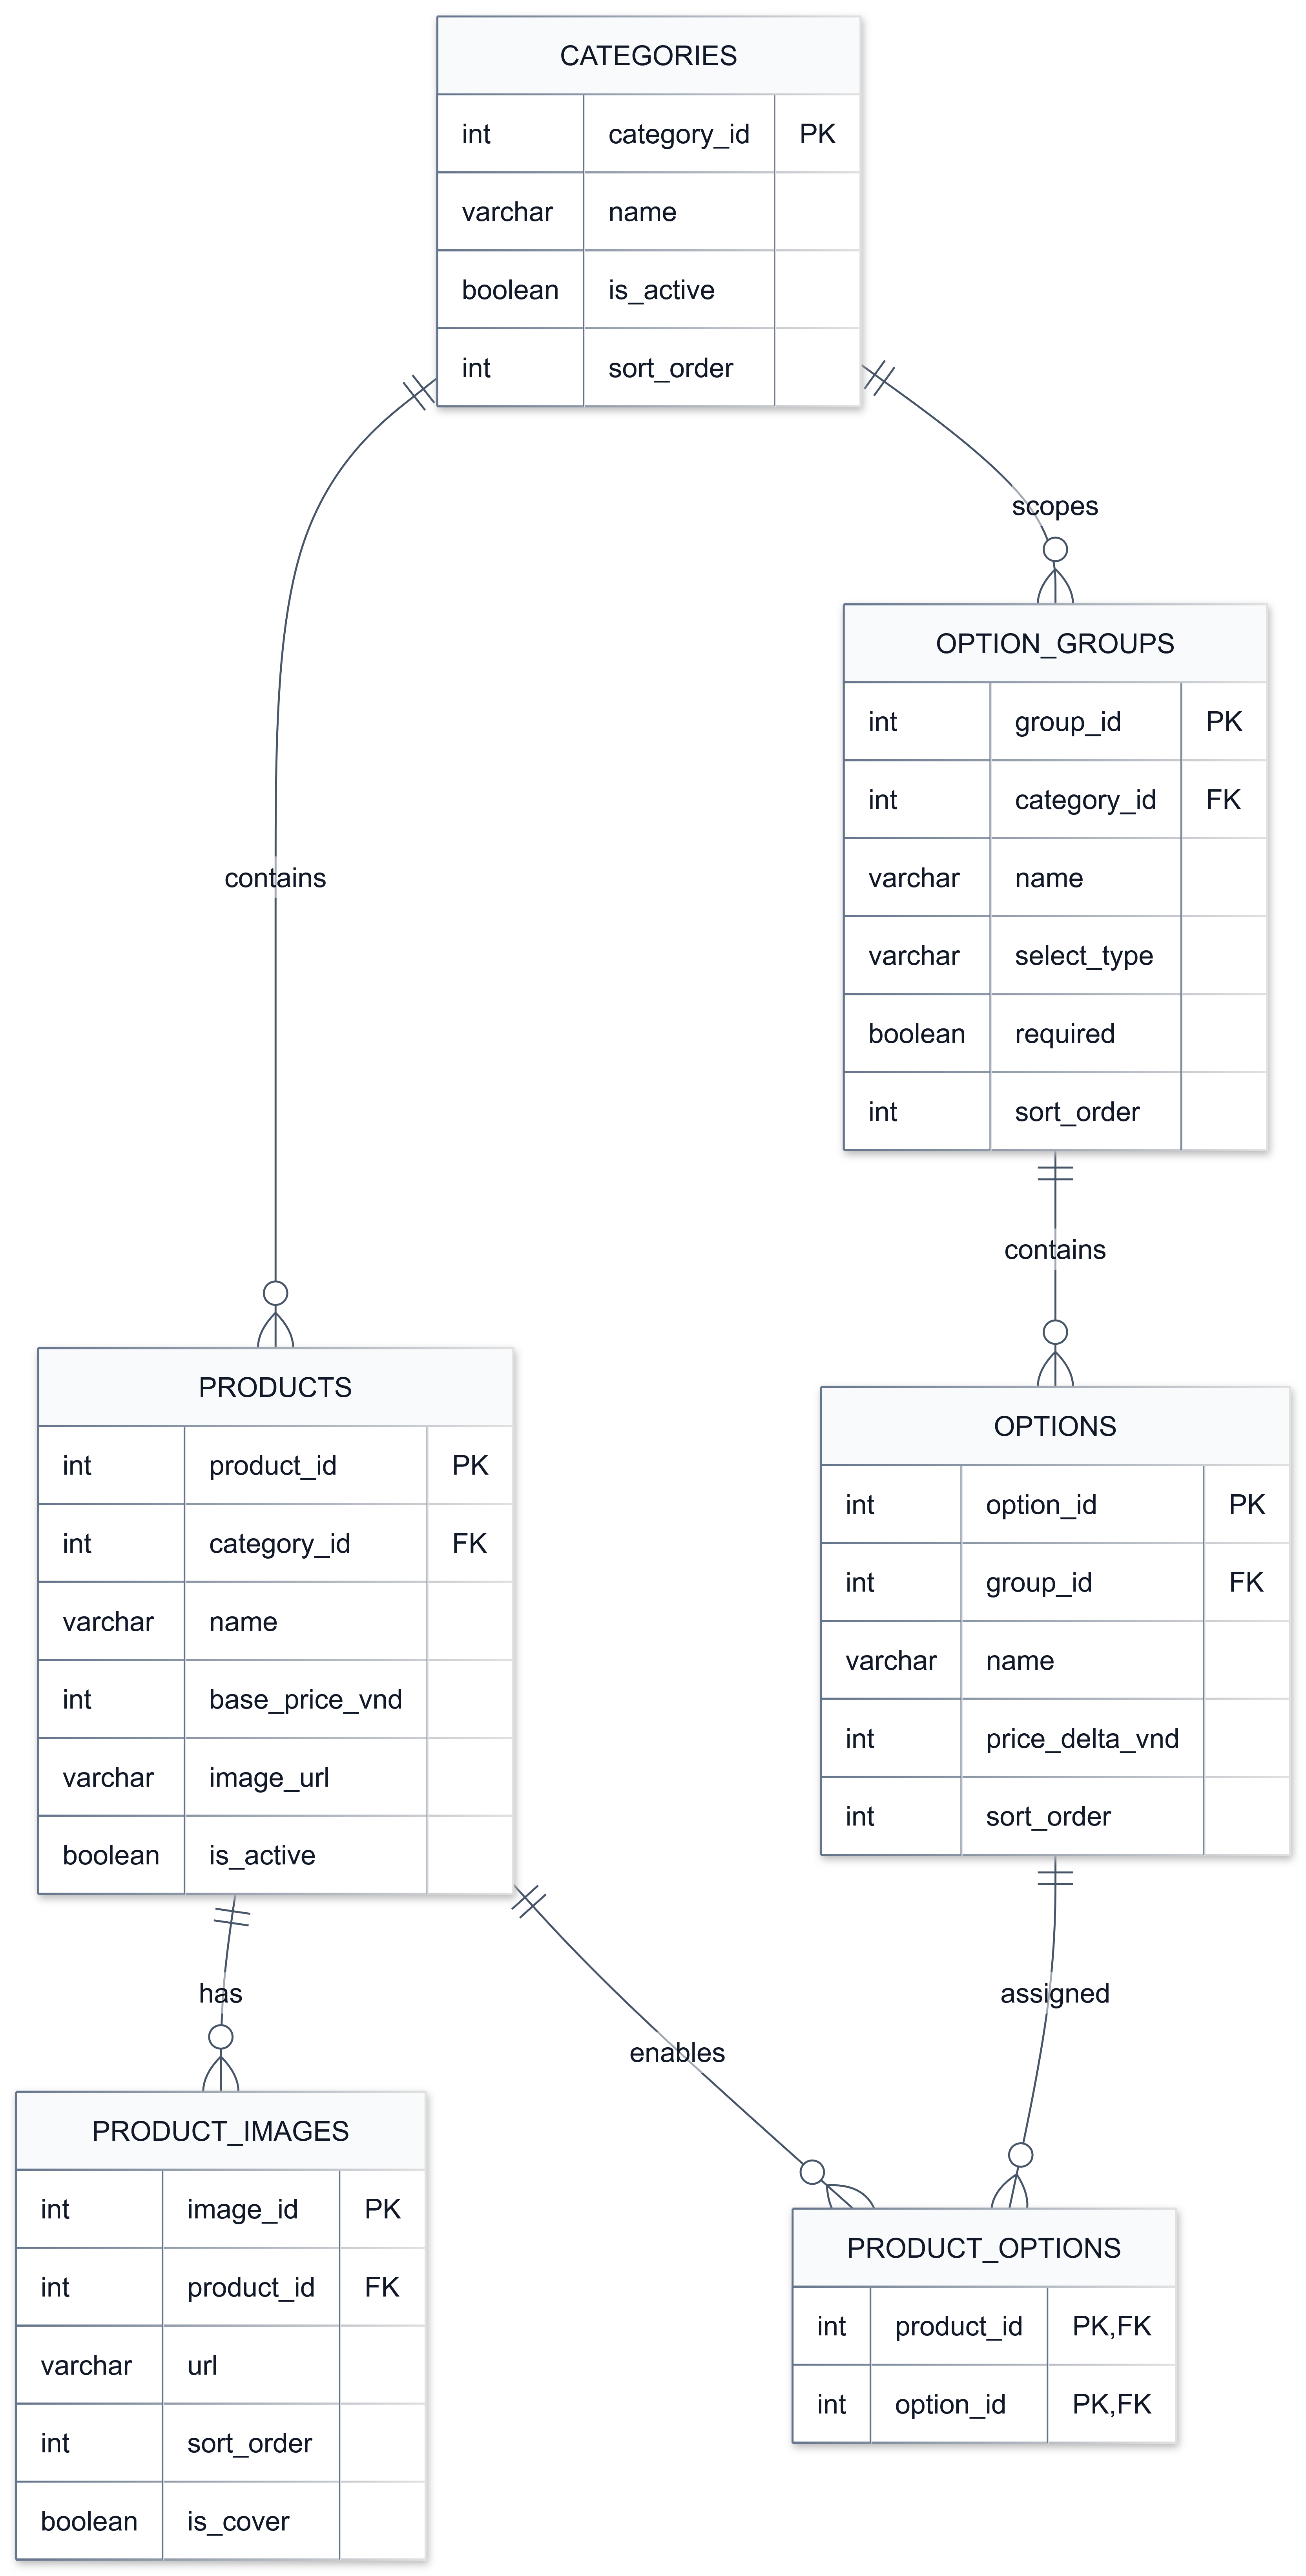
\includegraphics[width=0.86\textwidth,height=0.70\textheight,keepaspectratio]{latex_report/figures/database_catalog_options.png}
    \caption{Current catalog, image, and option-enablement relationships}
    \label{fig:database-catalog-options}
\end{figure}

\begin{figure}[htbp]
    \centering
    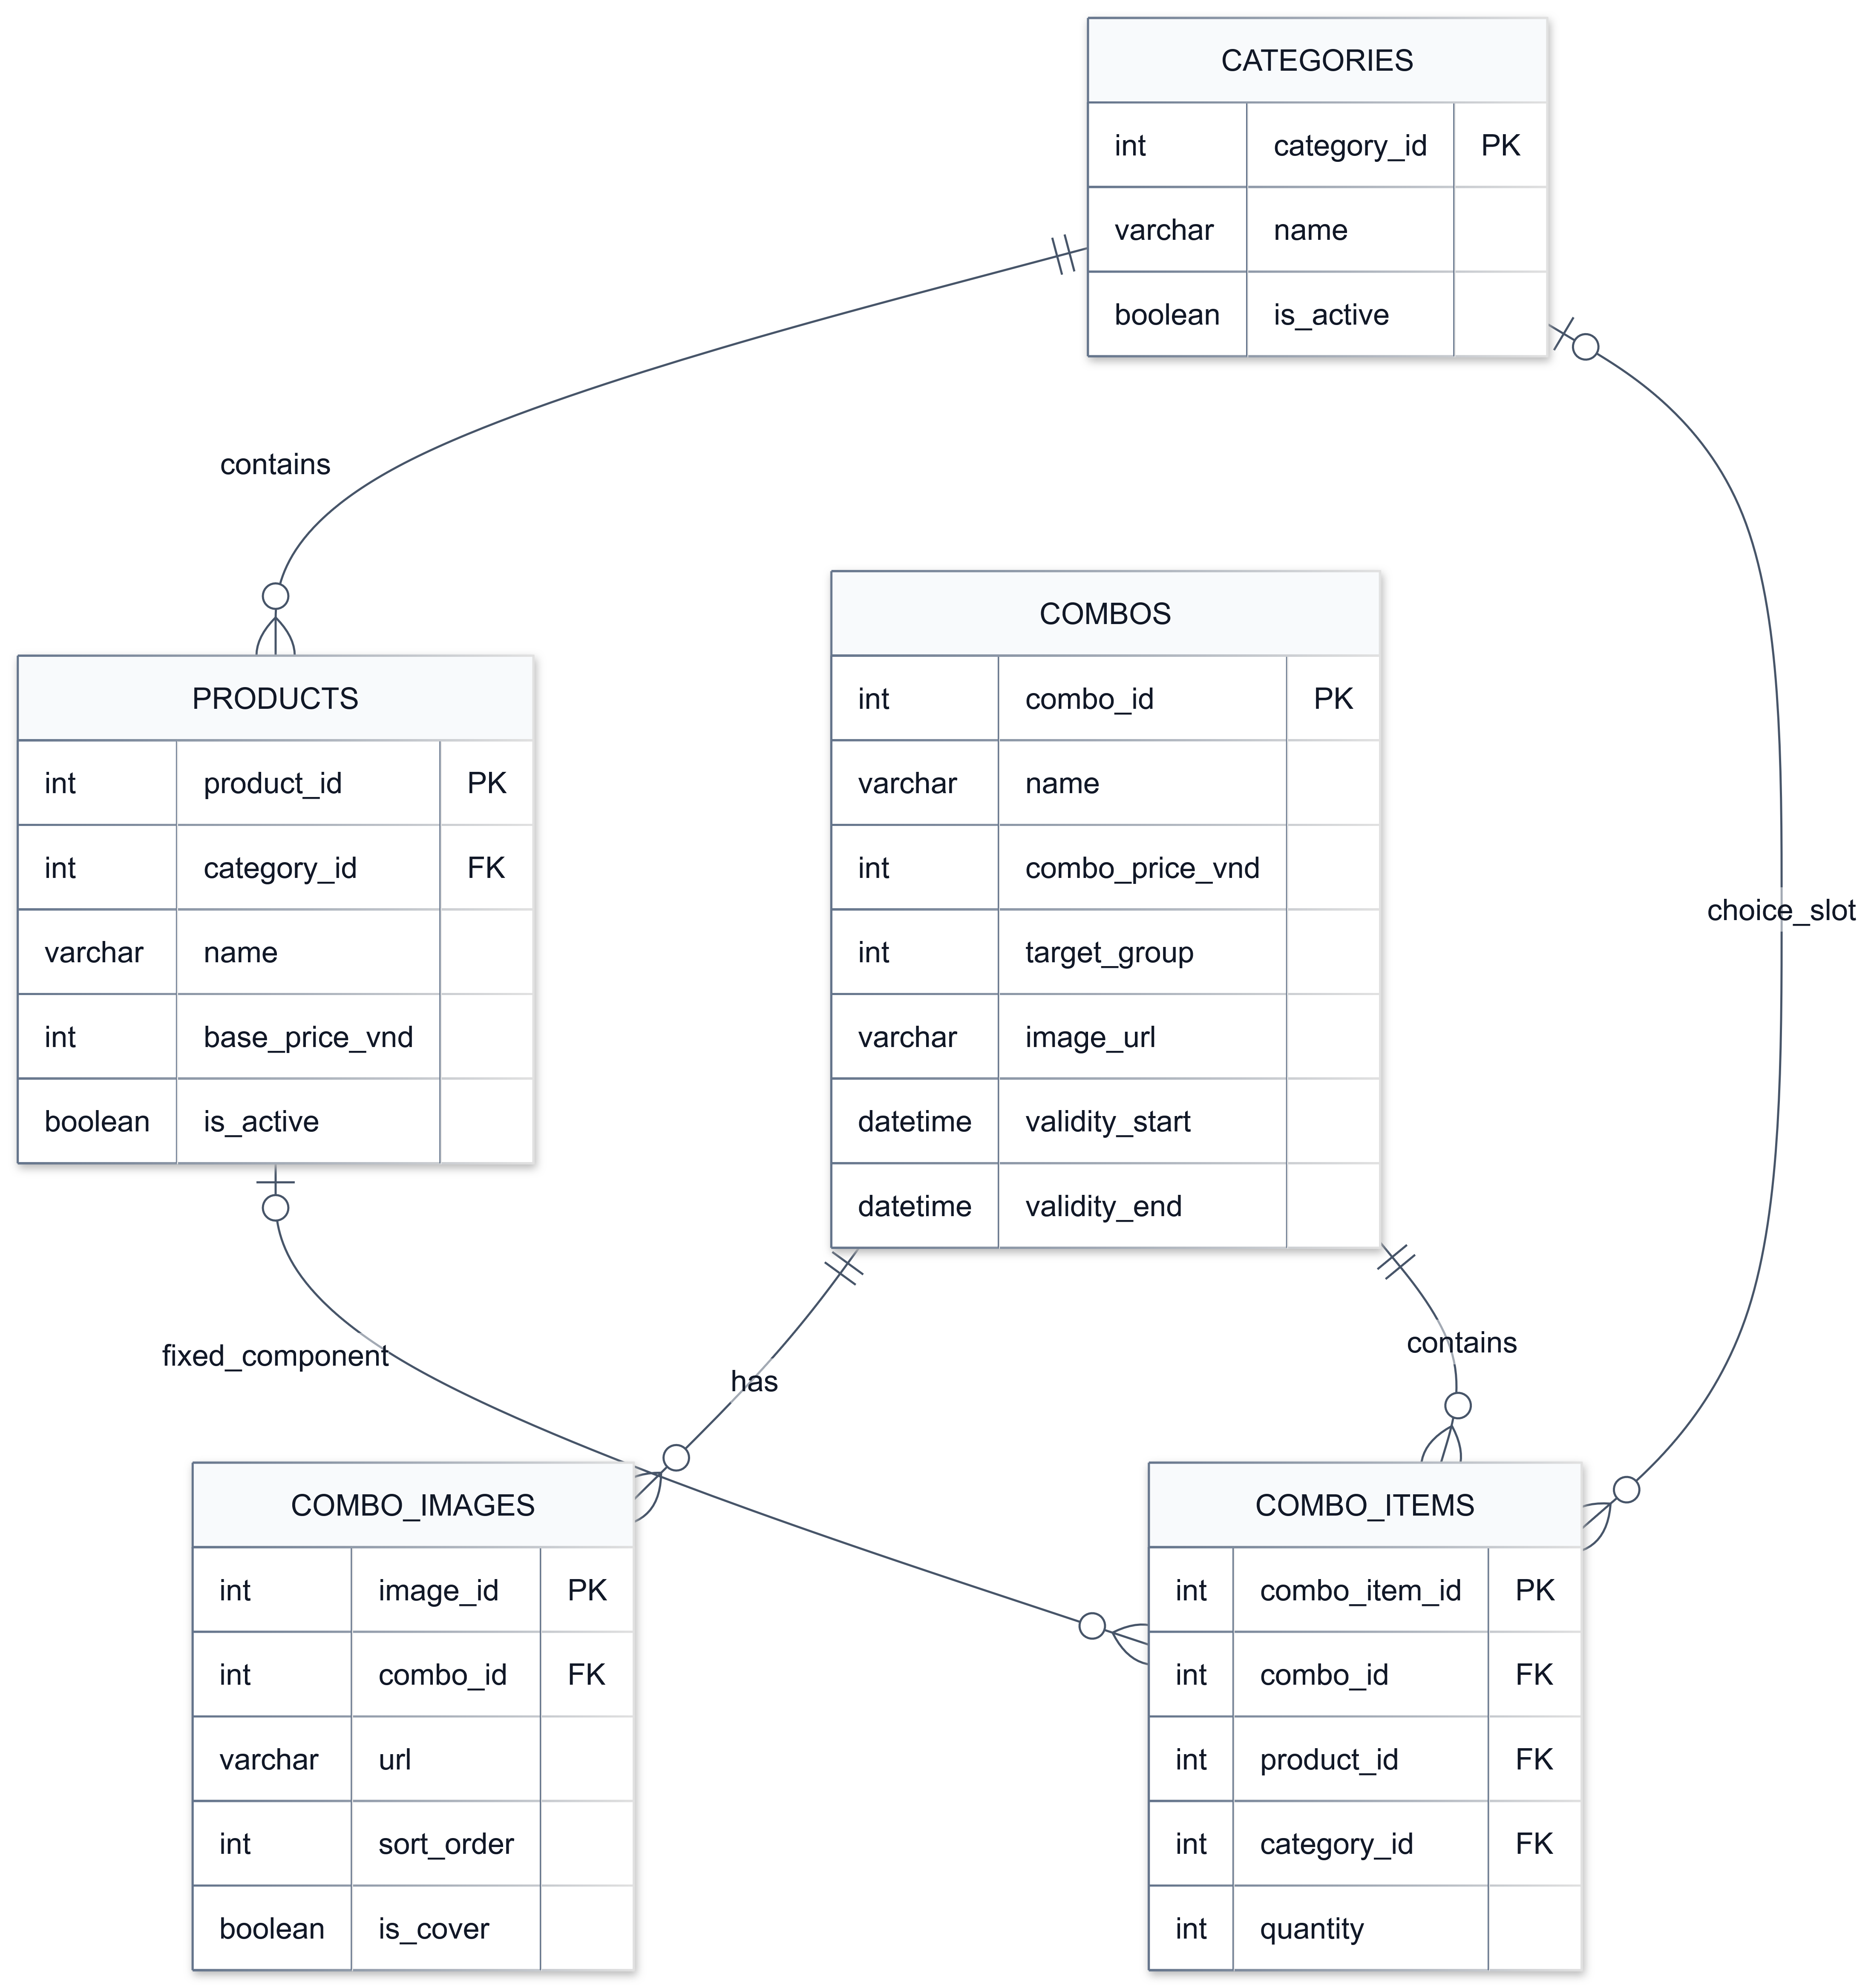
\includegraphics[width=0.86\textwidth,height=0.70\textheight,keepaspectratio]{latex_report/figures/database_combos.png}
    \caption{Current combo campaign, image, and choice-slot relationships}
    \label{fig:database-combos}
\end{figure}

\begin{figure}[htbp]
    \centering
    \includegraphics[width=0.90\textwidth,height=0.74\textheight,keepaspectratio]{latex_report/figures/database_orders.png}
    \caption{Current cart, order, tracking, and snapshot relationships}
    \label{fig:database-orders}
\end{figure}

At a high level, the most important relationships are:

\begin{itemize}
    \item each product belongs to one category;
    \item option groups are category-owned, and options belong to one option group;
    \item products enable a subset of options through the \texttt{product\_options} bridge;
    \item products and combos may each carry multiple gallery images through dedicated image tables;
    \item combos contain component rows, where each component is either a fixed product or a category-scoped choice slot;
    \item carts and cart lines preserve server-side pre-order state before order creation;
    \item orders contain multiple order items, and combo orders may decompose into parent and child order-item rows;
    \item order-item option selections are preserved as snapshots rather than live foreign-key references to mutable catalog options.
\end{itemize}

\subsection{Key integrity and business rules}

\subsubsection{Guest and registered-customer ordering}

The \texttt{orders.user\_id} reference is nullable. This allows the same order model to represent:

\begin{itemize}
    \item guest orders, which have no customer-account owner;
    \item customer orders, which are linked to a registered account.
\end{itemize}

This is a practical design because the client requires guest checkout as well as account-based features.

\subsubsection{Customization and option control}

The customization model is intentionally normalized. \texttt{option\_groups} define reusable logical groups such as sizes, crusts, or toppings, and are now scoped by category rather than treated as globally free-floating records. \texttt{options} define selectable choices and their price deltas. \texttt{product\_options} then determines which options are enabled for a given product. This avoids duplicating every option directly inside each product definition while still allowing per-product control.

\subsubsection{Combo modeling and choice slots}

Combo modeling evolved beyond a simple fixed bundle. The current schema supports an XOR-style combo component rule: a \texttt{combo\_items} row points either to a fixed \texttt{product\_id} or to a \texttt{category\_id} representing a customer's-choice slot. This is enforced through a check constraint in the current model. As a result, the database can support both rigid combos and partially customizable combo campaigns.

\subsubsection{Snapshot preservation in order history}

One of the most important database decisions is the use of \texttt{order\_item\_options} as a snapshot table. Each row stores the group name, option name, and price delta that applied at order time, without a foreign key to the live \texttt{options} table. This means administrators may later change or delete options without corrupting the historical meaning of past customer orders.

\subsubsection{Order-state and tracking history}

The order header stores the current visible lifecycle state, while \texttt{order\_tracking} stores historical state changes and related notes. This allows the application to present both the current status and a timeline of how the order reached that state. It also supports multi-actor workflow recording, since updates may originate from kitchen actions, administrative actions, system events, or transport callbacks, and the \texttt{note\_source} field records that origin explicitly.

\subsubsection{Kitchen read model}

The schema defines \texttt{kitchen\_queue\_view} as a SQL read model for queue prioritization. Rather than being a raw source-of-truth table, this object summarizes order data into a kitchen-oriented projection that can support priority-based processing behavior.
